\section{Motion, forces and energy}
\subsection{Physical quantities and measurement techniques}

Lengths can be measured using measuring tapes, rulers and micrometers.

A measuring cylinder can be used to find the volume of an irregularly shaped object. A volume
of liquid will first be taken in the measuring cylinder, which must fit the irregular object in
question. The object will then be submerged into the liquid, and we will measure the change in
volume reading of the liquid. For this case, note that $\SI{1}{cm^3} = \SI{1}{ml}$.

A scalar quantity has only a magnitude, and a vector quantity has magnitude and a direction related
with that magnitude. Vector quantities will be denoted in this text as $\vec{x}$. Some scalar
quantities are that of: distance, speed, time, mass, energy, and temperature. Some vector 
quantities follow: displacement, force, weight, velocity, acceleration, momentum, electric field
strength and gravitational field strength.

Vectors are represented as arrows pointing in space. Those arrows have a direction, and a length,
corresponding to the direction and magnitude of the quantity being represented by the arrows.

\begin{center}
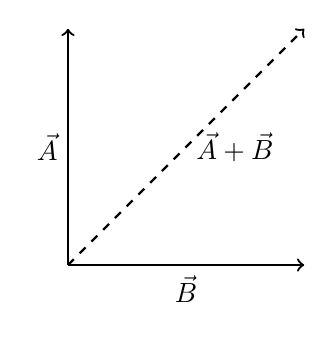
\begin{tikzpicture}

    % Centered Diagram: Vectors pointing away, A and B at 90 degrees
    \draw[thick, ->] (0,0) -- (3,0) node[midway, below]{$\vec{B}$};
	\draw[thick, ->] (0,0) -- (0,3) node[midway, left]{$\vec{A}$};
	\draw[thick, ->, dashed] (0,0) -- (3,3) node[midway, right]{$\vec{A} + \vec{B}$};

\end{tikzpicture}
\end{center}
The above diagram shows two vectors: $\vec{A}$ and $\vec{B}$ and their resultant vector or their 
sum: $\vec{A} + \vec{B}$. To find the magnitude of their sum, or $\left|\vec{A} + \vec{B}\right|$,
we can utilise the Pythagorean theorem:

$$\left|\vec{A} + \vec{B}\right| = \sqrt{ \left|\vec{A}\right|^2 + \left|\vec{B}\right|^2 }$$

\subsection{Motion}
Speed is the distance travelled by an object per unit time, and velocity is the change in 
displacement of an object per unit time. The displacement of an object is how far it is from a
given origin point. This results in the following equation:

$$ v = \frac{s}{t} $$
$$ \vec{v} = \frac{\vec{s}}{t} $$
where $s$ is displacement or distance, given the context, $v$ is velocity or speed respectively and
$t$ is time taken to cause the corresponding change in displacement or to travel $s$ distance.

The average speed of an object is given by the total distance it travelled over the total time it
took:
$$ \textrm{average speed} = \frac{\textrm{total distance travelled}}{\textrm{time taken}} $$

Acceleration is a vector which is the rate of change of velocity with respect to time, as seen in 
the equation:
$$\textrm{acceleration, } a = \frac{\Delta v}{\Delta t} $$

Uniform acceleration arises when the value of acceleration is unchanging. It causes a linear 
change in velocity with change in time, as seen in:
$$ \Delta v = a (\Delta t) $$
A non-constant, i.e. changing value of acceleration results in a non-linear change in velocity, as
seen by the same equation if the values of $a$ is different for values of $t$.

A deceleration is simply negative acceleration, negative acceleration causes decrease in velocity.
A deceleration of \SI{9}{ms^{-2}} is equivalent to an acceleration of \SI{-9}{ms^{-2}}.

The values of speed, distance and velocity can all be plotted against time to see graphically, the
relationships between all these variables.

\begin{center}
\begin{tikzpicture}

% Speed-time graph
% Axes
\draw[->] (0,0) -- (7,0) node[below] {$t$};
\draw[->] (0,0) -- (0,3) node[left] {$v$};

% Constant acceleration
\draw[thick] (0,0) -- (2,2);

% Zero acceleration (constant speed)
\draw[thick] (2,2) -- (4,2);

% Deceleration
\draw[thick] (4,2) -- (6,0);

% Dashed lines to x-axis
\draw[dashed] (2,2) -- (2,0) node[below] {$t_1$};
\draw[dashed] (4,2) -- (4,0) node[below] {$t_2$};
\draw[dashed] (6,0) -- (6,0) node[below] {$t_3$};

% Origin label
\node at (-0.2,-0.2) {$O$};

\end{tikzpicture}

velocity-time, $v$-$t$, graph.
\end{center}
In the above graph, a stopwatch is started at time, $t = \SI{0}{s}$. The velocity of an object
is measured at certain time intervals, using the data from which, the graph is drawn. 

For 
$0 \le t \le t_1$, the graph shows a straight line. This means that the gradient of the curve must
be constant. By definition, acceleration is the gradient of velocity with respect to time since
it is the rate of change of velocity with respect to time. So a straight line in a $v$-$t$ curve
shows that acceleration is constant, i.e., uniform. Otherwise, the acceleration can be said to be
non-uniform. For $t_1 \le t \le t_2$, the line is parallel to the horizontal axis. This means the
gradient, $a$, equals 0. Note that, the area under a $v$-$t$ graph gives distance or displacement,
given context, since the product of the units of the axes, \SI{}{(ms^{-1})(s)} = \SI{}{m}, gives
the unit of distance. Lastly, $t_2 \le t \le t_3$ is a downward sloping line, meaning the 
acceleration is negative, and negative acceleration is decleration.

\begin{center}
\begin{tikzpicture}

% Speed-time graph
% Axes
\draw[->] (0,0) -- (7,0) node[below] {$t$};
\draw[->] (0,0) -- (0,3) node[left] {$s$};

% Constant acceleration
\draw[thick] (0,0) -- (2,2);

% Zero acceleration (constant speed)
\draw[thick] (2,2) -- (4,2);

% Deceleration
\draw[thick] (4,2) -- (6,0);

% Dashed lines to x-axis
\draw[dashed] (2,2) -- (2,0) node[below] {$t_1$};
\draw[dashed] (4,2) -- (4,0) node[below] {$t_2$};
\draw[dashed] (6,0) -- (6,0) node[below] {$t_3$};

% Origin label
\node at (-0.2,-0.2) {$O$};

\end{tikzpicture}

distance-time, $s$-$t$, graph.
\end{center}
